\documentclass[conference]{IEEEtran}

\usepackage{amsmath}
\usepackage{cite}
\usepackage{graphicx}
\usepackage{color}
\newcommand{\unit}[1]{\ensuremath{\, \mathrm{#1}}}

\graphicspath{{plots/}}

\begin{document}

\title{Efficient Extraction of Regional Subsets from Massive Climate Datasets
using Parallel IO}

\author{
\IEEEauthorblockN{
    Jeff Daily\IEEEauthorrefmark{1},
    Karen Schuchardt\IEEEauthorrefmark{1} and
    Bruce Palmer\IEEEauthorrefmark{1}
}
\IEEEauthorblockA{
    \IEEEauthorrefmark{1}
    Pacific Northwest National Laboratory\\
    jeff.daily,karen.schuchardt,bruce.palmer@pnl.gov
}
}

\maketitle

% For peer review papers, you can put extra information on the cover
% page as needed:
% \ifCLASSOPTIONpeerreview
% \begin{center} \bfseries EDICS Category: 3-BBND \end{center}
% \fi
%
% For peerreview papers, this IEEEtran command inserts a page break and
% creates the second title.  It will be ignored for other modes.
\IEEEpeerreviewmaketitle

\begin{abstract}
\label{section:abstract}

The size of datasets produced by current climate models is increasing rapidly
to the scale of petabytes.  To handle data at this scale parallel analysis
tools are required, however the majority of climate analysis software remain
at the scale of workstations.  Further, many climate analysis tools adequately
process regularly gridded data but lack sufficient features when handling
unstructured grids.  This paper presents a data-parallel subsetter capable of
correctly handling unstructured grids while scaling to over 2000 cores.  The
approach is based on the partitioned global address space (PGAS) parallel
programming model and one-sided communication.  The paper demonstrates that IO
remains the single greatest bottleneck for this domain of applications and
that parallel analysis of climate data succeeds in practice.

\end{abstract}

\section{Introduction}
\label{section:introduction}

Parallel programming is needed to analyze the size of output data produced by
today's climate models.\cite{MODSIM07:LOT}  A single snapshot of Randall's
Global Cloud Resolving Model will produce terabytes of data\cite{GCRM}; the
analysis of even a modest time series of this data will quickly overwhelm
today's software and traditional climate analysis systems.  For these data
sizes, I/O bandwidth represents the single greatest bottleneck for analysis
tools.  Parallel software leveraging parallel file systems must be used to
process this data, however current climate analysis tools are at most task
parallel and rely on a single data reader.\cite{CDAT}\cite{CDO}\cite{NCO}

Many climate analysis tools robustly handle the manipulation and display of
regularly gridded data.  However, these same applications lack sufficient
features when handling unstructured or irregular grids such as the geodesic or
cubed sphere\cite{CUBE}.  Unstructured grids are gaining popularity, further
widening the gap between current software and these types of models.  For
unstructured grids it is necessary to provide more information about the
topology of the grid and maintain the integrity of this topology information
in the face of data culling.

Regular grids allow for the topology to be implicitly defined by how
the data is stored; coordinate variables are generally monotonic and cell
neighbors are adjacent both logically and in memory. These assumptions allow
for operations over regular grids which are otherwise more difficult to
perform over unstructured grids. In the case of partitioning these grids for
data parallel processing, unstructured grids will often have more of the
logically adjacent cells scattered across memory partitions than in the
regular case.

Subsetting is a fundamental capability for any analysis tool and allows users
to operate over the regions of the data in which they are interested. The
subsetting operation is useful as part of a larger operation over the data,
such as for obtaining regional averages, but is also useful to post-process
data into a new dataset such that the cost of subsetting can be amortized
across future operations over the same region. Further, as the size of
datasets grow subsetting is important to reduce the data to a size that
traditional analysis tools are capable of handling. 

In this paper, we present a parallel tool for subsetting very large geodesic
climate data in parallel while preserving the explicit topology.  The code is
built using the Global Arrays (GA) toolkit which provides an efficient and
portable "shared-memory" programming interface for distributed-memory
computers and features truly one-sided communications.\cite{GA}  GA
traditionally deals with dense arrays, however its sparse data operations as
well as its one-sided operations allow for efficient subsetting over
unstructured grids.

The primary contributions of the paper are:
\begin{itemize}
\item A parallel subsetter of geodesic data based on the partitioned global address space programming model and one-sided communications
\item A novel algorithm for the maintenance of unstructured grid data
\item A novel algorithm for the subset and even distribution of unstructured grid data
\item Evaluation showing IO to be the greatest bottleneck in scaling these types of applications
\end{itemize}

The paper is organized as follows.  Section \ref{section:requirements}
describes the requirements while \ref{section:design} describes the design of
the subsetter, its algorithms, and how GA's unique features were leveraged.
Section \ref{section:implementation} briefly describes how the subsetter was
implemented.  Section \ref{section:evaluation} presents our experimental design
and the performance characteristics of the subsetter on nearly full-scale data
set sizes of model data up to a resolution of 4Km.  We present the
capabilities under development as well as the capabilities we would like to
see in section \ref{section:future}.  Finally, section
\ref{section:conclusion} presents our conclusions.

\section{Requirements}
\label{section:requirements}

The requirements for our software stem from the growing need for parallel
analysis in the domain of climate science\cite{MODSIM07:LOT} but also from
the use of the geodesic grid.

\subsection{Geodesic Grid}
\label{subsection:grid}

Until recently, climate and weather models have primarily been simulated on
structured grids that divide the latitude and longitude axes in even
increments, resulting in logically structured simulation grids. Standard
conventions for describing this data in the NetCDF data model have been
formalized by the Climate and Forecast (CF) conventions. CF defines
conventions and metadata standards that enable both human and computer
interpretation of the data.  Human interpretation is supported through the use
of standard names while definition of spatial and temporal properties of the
data have enabled an extensive set of tools for data manipulation and display
such as \cite{NCO}, \cite{OPeNDAP}, and \cite{FERRET}.  The CF Conventions
have been evolving to support many variations of structured grids including
Orthographic, Polar stereographic, Transverse Mercator, and many others . 

The GCRM uses a geodesic grid.  The geodesic grid is created by recursively
bisecting an icosahedron of 20 triangular faces and twelve vertices and
projecting the resulting faces onto a unit sphere.  The resulting vertices
represent the centers of hexagonal grid cells with the exception of twelve
pentagons (the centers of the original twelve vertices.) See
\ref{fig:geodesic} for an example of the first stage of bisection and
projection, followed by the definition of one of the hexagons.  Further
details can be found in \cite{GEODESIC}.

\begin{figure}[!t]
\center
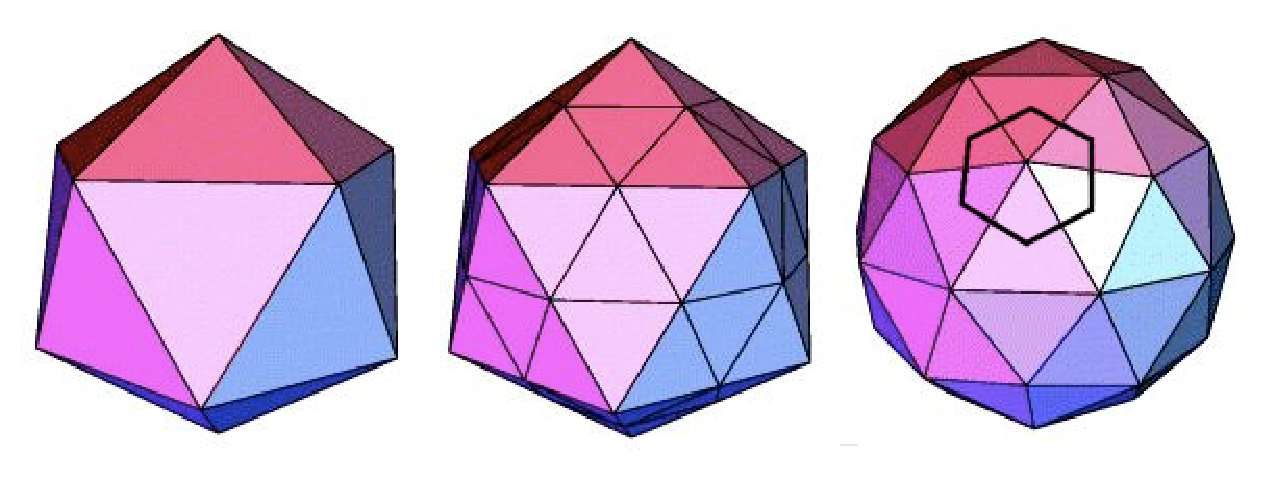
\includegraphics[width=3.5in]{images/geodesic2}
\caption{First stage generation of the geodesic grid}
\label{fig:geodesic}
\end{figure}

From the previous description, it can be seen that the geodesic grid used by
the GCRM is fairly regular. However, the horizontal dimension has some
important properties in common with unstructured grids: the grid coordinates
are not monotonic and simple conventions are not available for identifying the
neighbors of all cells.  As a consequence, it is necessary provide more
information about the topology of the grid. Other unstructured grids such as
triangular, cubed sphere \cite{CUBE}, and arbitrary unstructured polygons are
also being applied to various models.  There is a recognized need to extend
the CF conventions to unstructured grids so that general data analysis,
regridding, and display tools can be developed. As yet, no such standard
exists.  Balaji has cataloged a number of unstructured grids \cite{Balaji} and
proposes a tiling approach to describing grids.  The tiling approach supports
embedded and nested grids but has been slow to gain momentum, in part due to
its complexity.  In the ocean modeling community, workshops to discuss
standards have taken place \cite{UGRIDS}, however, these efforts are still in
the early stages of development and acceptance.   Lacking a standard,
development of general purpose tools has been slowed.  However some
preliminary tools and approaches have progressed by focusing on the in-memory
operations and abstracting the data loading from the processing \cite{UGRID}. 

Although the geodesic grid is fairly structured, we choose to represent it in
an unstructured way.  Each of the grid's cells, corners, and edges are
uniquely indexed from zero.  For a given positive integer $R$, there are $N =
10 \times 2^{2R} + 2$ cells, $C = (N-2) \times 2$ corners, and $E = (N-2)
\times 3$ edges.  Increasing the value of $R$ increases the resolution of the
model.  For example, a value of $R=10$ is approximately 8Km while $R=11$ is
approximately 4Km.  The cells, corners, and edges are represented as
dimensions within a NetCDF file.

The horizontal topology describes the connectivity relationships between
cells, nodes, and edges, all of which may have associated 3D data.  The
topology consists of three primary arrays: a mapping between cells and cell
corners, a mapping between cells and cell edges, and a mapping between edges
and corners.  Because neighbor lists are important for visualization programs
but difficult to generate in the general case, they are included as part of
the topology as the \verb+cell_neighbors(cells,neighbors=6)+ variable.  The
vast majority of cells are hexagons, so we have
\verb+cell_corners(cells,cellcorners=6)+,
\verb+cell_edges(cells,celledges=6)+, and
\verb+edge_corners(edges,edgecorners=2)+.  For the twelve pentagons, the last
values in these arrays are repeated but could just have easily been set to a
negative index.

The horizontal geometry describes the longitude and latitude location of each
object.  That is, there is one latitude and one longitude array for each of
the topology objects (cell centers, corners, and edges).

The vertical grid consists of layers sandwiched between interfaces with the
number of layers equal to the number of interfaces minus 1.   Because grid
variables are associated with both locations, layers and interfaces are
defined as dimensions.  They can be thought of as two distinct vertical grids
from a representation standpoint.

The data model is designed to support efficient model output, fully describe
the grid topology, and provide the sufficient information for tessellation to
triangles for 3D visualization.  The approach taken with the model is to adopt
the CF conventions to the extent possible and adopt early ideas circulating
within the community.  However, as many of the details have not been decided,
custom data analysis tools are currently required.

\subsection{Data Parallelism}

Larson, Ong, and Tokarz note that the current popular climate data analysis
packages remain single-processor applications which lack the memory required
to handle large data volumes as well as the processing power to analyse the
data in a timely fashion.\cite{MODSIM07:LOT}  Although they emphasize using
OpenMP as a first step toward parallism, we instead emphasize using a
distributed data model first.  Well designed communication libraries such as
MPI may already take advantage of shared-memory parallelism within a compute
node or multi-core desktop computer.

The data parallelism offered by libraries such as MPI or Global Arrays is
absolutely necessary to handle the size of data of modern climate models.  An
edge data variable of the geodesic grid at an approximate resolution of 4Km
and 100 levels is nearly $10 \times 2^{2R} \times 3 \times 100 \times 4
\unit{bytes} \approx 50 \unit{gigabytes}$ in size.  Even a modest number of
these variables will surpass the memory available in most desktop systems and
even some small clusters.

\subsection{Fast IO}

For data of this size, efficiently reading from and writing to disk requires
the use of parallel IO libraries such as Parallel NetCDF\cite{PNETCDF} or the
HDF5/NetCDF4\cite{HDF5}\cite{NETCDF}, both of which are in turn built on top
of the MPI-IO libraries\cite{MPIIO}.  Currently, GCRM output is stored in
netCDF\cite{NETCDF} files, a format for storing array-oriented
machine-independent data.

\subsection{Dataset Abstraction}

Model output is often distributed across many files for a given model run.
There are any number of schemes for organizing so many files e.g. one variable
per file with multiple timesteps per file, separating out the grid into a
separate file, one timestep per file with multiple variables.  The
reconstitution of these files into a logical set of variables and metadata is
an established practice.\cite{NcML}\cite{THREDDS}  We emphasize that the
aggregation of files into an abstract dataset is required in order to operate
on the data itself.  Operations on a dataset are more intuitive than needing
to know the addling details of which files hold which variables.

\subsection{Maintenance of Topology Variables}

Regular grids such as the cartesian, rectilinear, or curvilinear lend
themselves to representations as multidimensional arrays such that logically
adjacent cells are either adjacent in memory or can be located via a
shape-based index calculation.  Although some attempt is made to keep
logically adjacent cells nearby in memory, geodesic grids do not have the
luxury of using relatively simple shape-based index arithmetic to locate
neighbors.

The topology variables mentioned in \ref{subsection:grid} are not unique to
our grid; any grid could be described using a similar set of variables.
However, since topology is often implicitly defined by other grids, these
variables are not correctly handled by current software.  When a subset
occurs, the indices of these variables must be updated to reflect the
remaining corners, edges, and cells.

\subsection{Maintain Integrity of Entire Grid Cells}

Howe and Maier detail the properties of well-formed grids in \cite{UGRID}.
Proper subsets should maintain the same well-formed properties of the original
in order to remain useful to further analysis.  Therefore, the cell and its
surrounding corners and edges must remain intact during a subset.

\section{Design}
\label{section:design}

In this section we describe the design of our classes and algorithms based on
the requirements established in \ref{section:requirements}.

\subsection{How to Run the Subsetter}

The success of the NetCDF Operators and similar tools demonstrate the need for
user-ready applications for the analysis of their data while the success of
tools such as CDAT validate the need for a scriptable interface and customization of
basic and advanced operators.  We plan to provide both the scriptable
interface as well as a set of predefined tools.

The subsetter is the first in a series of planned parallel command-line tools
based on unstructured grids and the PGAS programming model.  It takes
arguments specifying specific variables (-v) or dimension ranges (-d) to
extract, or at a higher level a latitude and longitude bounding box (-b).  In
this way it is most akin to the NetCDF Operators' "kitchen sink" application.
Example usage looks like: \begin{itemize} \item mpiexec -np 128 subsetter -b
20,-20,160,90 -v vorticity january.nc february.nc MJO\_vorticity\_janfeb.nc
\item mpiexec -np 64 subsetter -b 90,0,180,-180 -d levels,1,5 geopotential.nc
\end{itemize}

\subsection{Dataset Abstraction}

The subsetter minimally supports two forms of input file aggregation, either
across a specified dimension e.g. time or by taking the union of all input
files such that duplicate dimensions and variables within later files are
ignored.  These forms of aggregation are modeled after what is available when
using NetCDF Markup Language.\cite{NcML} NcML input is not directly supported
at this time but is planned for a future release. 

\subsection{Parallel IO Abstraction}

IO operations are hidden behind abstract base classes.  Any IO library can be
supported.  This is similar to how the Java NetCDF library works
\cite{JavaNetCDF}.  Further, differing IO strategies using the same IO library
can also be developed behind the same API.  The use of Parallel NetCDF was
selected because of the ubiquity of the NetCDF libraries and data format in
climate applications.

\subsection{The Global Arrays Library}

The partitioned global address space (PGAS) programming model assumes a global
address space which is partitioned such that each process is associated with a
local portion of the space.  One-sided communication allows a process to
access another process's address space without any explicit participation by
the latter process.  Such communication can reduce synchronization, reduce
data movement, and can simplify programming.  The Global Arrays (GA) library
supports both models.

The subsetter was built using the GA library for the wealth of features it
provides which are tailored to our problem domain.  GA provides a distributed
dense multidimensional array programming abstraction and the data we will be
operating over is stored as dense arrays within NetCDF files.  It should be
noted that dense distributed arrays would also work well for regularly gridded
data.  However, due to the use of unstructured grid data, the algorithm for
subsetting the data will look quite different than for the structured case.
Recall that for unstructured grids, logically adjacent cells are not
necessarily adjacent in memory.  In order to evenly distribute a subset, a
single process will need to send a varying amount of data to any number of
other processes.  Certainly a collective operation could be considered, but GA
provides the necessary functionality without needing any explicit cooperation
from any other process.  Any given process will simply put the section of the
subset into the remote process's memory.

There are certain GA one-sided operations which are tailored for use on
one-dimensional arrays which are prevalent within our data.  These operations
include \verb=GA_Patch_enum=, \verb=GA_Scan_add=, \verb=GA_Scan_copy=,
\verb=GA_Pack=, and \verb=GA_Unpack=.  Those operations have been demonstrated
in the computation of sparse matrix multiplication\cite{GA} but are equally
useful in the manipulation of unstructured grids.  The remaining GA operations
are N-dimensional and include \verb=NGA_Scatter=, \verb=NGA_Gather=,
\verb=GA_Put=.  Those operations are useful for redistributing the subset
data.

\subsection{The Algorithms}

The one-sided communications and PGAS model supported by GA allowed us to
develop some novel algorithms for the manipulation of unstructured grids.  In
this section we diagram and describe the algorithms we developed.  The vast
majority of functionality within the subsetter is provided by either PnetCDF
or GA.  GA allocates and evenly distributes the arrays which are then filled
with data by PnetCDF.  GA operations are then used to prepare the data for
packing at which point a custom n-dimensional packing routine is used.  The
packed, evenly-distributed data is then written back to disk using PnetCDF.
Of these algorithms, the novel ones include reindexing the masks, reindexing
the topology variables, and the n-dimensional pack routine.

Each dimension of the data has two arrays associated with it, a bitmask and an
integer array representing the new indices of the dimension in case of a
subset.  For instance, if any of the bits are turned off, the corresponding
indices of the index array will have negative values.  The remaining values of
the index array will increase monotonically, skipping the negative or masked
indices.  The bitmasks are generated based on a rectangular latitude and
longitude region specified on the command-line, or by specifying one or more
indices of a dimension to select.  Although a rectangular region is currently
used for simplicity, once translated the bitmasks allow for arbitrary subsets
to be defined.  These bitmasks are then used to evenly distribute the
resultant subset across all processes.  Note that these bitmask and associated
index arrays are one-dimensional and distributed.

\subsubsection{Partial Sum}

\begin{figure}[!t]
\center
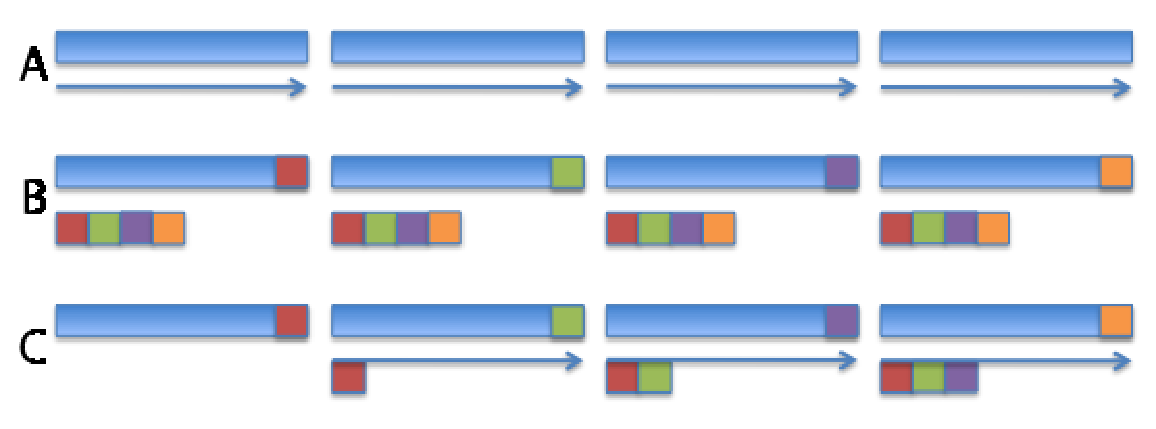
\includegraphics[width=3.5in]{images/partialsum_label}
\caption{Distributed partial sum on a 1-D array}
\label{fig:partialsum}
\end{figure}

A partial sum of the index array associated with each dimension is useful for
later determining where subset data is to be placed.  That feature will be
explained in more detail in \ref{section:alg_pack}.  The partial sum operation
here is semantically similar to the one found in the C++ STL\cite{CXXSTL}.  It
computes a series of sums over an array from the first element through the
\emph{i}th element and stores the result of each such sum in the \emph{i}th
element of a destination array.

The partial sum is computed by first performing partial sums of each local
portion of the source array.  This operation is represented by
\ref{fig:partialsum} A.  The last value of each local sum is then collectively
distributed to each process as seen in \ref{fig:partialsum} B.
\ref{fig:partialsum} C is the last step where each local portion adds the last
values of each process's sum which come before.

\subsubsection{Reindexing of Dimension Index}

\begin{figure}[!t]
\center
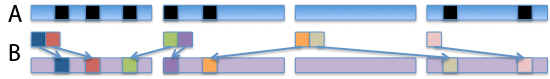
\includegraphics[width=3.5in]{images/unpack_label}
\caption{Reindexing of a Dimension Index}
\label{fig:unpack}
\end{figure}

Creating the index array associated with a mask requires three specific GA
operations, \verb=GA_Fill=, \verb=GA_Patch_enum= and \verb=GA_Unpack=.  The
mask array is represented in \ref{fig:unpack} A.  \verb=GA_Fill= fills the
index array, the bottom array in \ref{fig:unpack} B,  with a value of $-1$.  A
second array is created after each process counts how many masked bits are
present and collectively sums to get the size of the array to create.
\verb=GA_Patch_enum= enumerates the values in the second array starting from
zero with an increment of 1.  The enumerated array is shown in
\ref{fig:unpack} B.  \verb=GA_Unpack= expands the enumerated array values into
the filled array based on the associated mask array, seen as \ref{fig:unpack}
B.

\subsubsection{Reindexing of Topology Variables}

\begin{figure}[!t]
\center
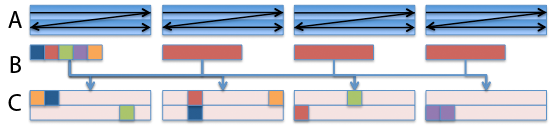
\includegraphics[width=3.5in]{images/reindex_label}
\caption{Reindexing of Topology Variables}
\label{fig:reindex}
\end{figure}

Recall that the topology variables are those which map from one index to
one or more other indices such as from a cell index to each of its corner
indices.  A typical subset operation reduces the number of cells, corners, and
edges within the grid, so it is important to maintain the integrity of these
mapping arrays such that they map to real indices.

The reindexing of the topology variables relies on the recalculated index
array of the associated domain.  For example, when reindexing the mapping from
edges to corners, the recalculated corners index array is required.  The
mapping values represent indices into the recalculated index array.  The
mapping arrays are iterated over to gather the required indices for the
subsequent GA routine \verb=NGA_Gather= to query, represented in
\ref{fig:reindex} A.  The \verb=NGA_Gather= routine gathers array elements
from a global array into a local array.  In this each process gathers the new
values for the mapping from the index array (\ref{fig:reindex} B) and
then appropriately replaces the old mapping values in \ref{fig:reindex} C.

\subsubsection{N-Dimensional Pack}
\label{section:alg_pack}

\begin{figure}[!t]
\center
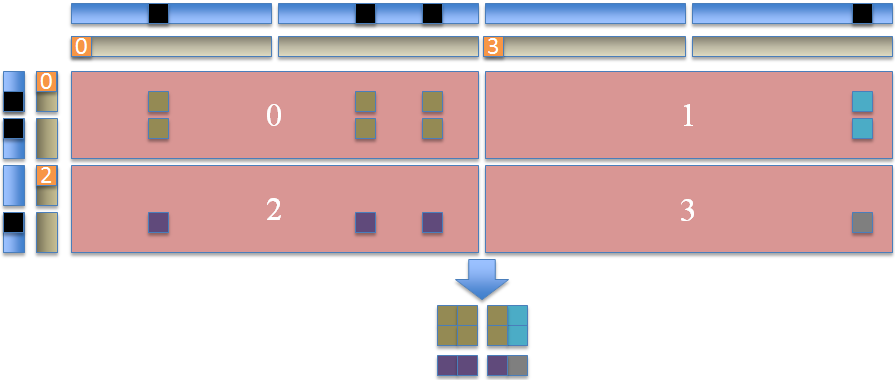
\includegraphics[width=3.5in]{images/pack}
\caption{Pack}
\label{fig:pack}
\end{figure}

The goal of the pack routine is to evenly distribute the subset destination
array from the already evenly distributed source array.  The subset is
specified using mask arrays, one for each dimension of the source array.  The
problem lies with where to put the data once each process computes its portion
of the subset; each process would need to know a priori the size of the
subsets that logically come before their own computed portion and
\verb=NGA_Put()= their data after then.

The partial sum of the mask array is a convenient solution to this problem.
Each process owns a portion of the source array in terms of the global address
space of the array.  For each dimension, the value in the corresponding
partial sum array at the index represented by the lowest index owned by each
local portion describes where to put the subset data.

Figure \ref{fig:pack} should clarify this.  In the figure, the blue arrays
represent both the mask arrays as well as the partial sum arrays.  The masked
bits are indicated in black.  Each of the four processes query the partial sum
arrays using \verb=NGA_Get()= at the corresponding locations indicated in
orange and the small blue arrows.  Now knowing where to put their subset data,
each process can \verb=NGA_Put()= their portions resulting in the subset
array.

\section{Evaluation}
\label{section:evaluation}

All tests were performed on the Franklin Cray-XT4 supercomputer\cite{franklin}
located at NERSC\cite{NERSC}.  The Franklin supercomputer features 9,572
Opteron 2.3 gigahertz quad core processors with 2 gigabytes of memory per
core.  Its Lustre parallel file system supports a theoretical peak of 16
gigabytes/second to each of two /scratch file systems.

In order to evaluate the scalability of our subsetter we performed strong
scaling tests. Data from the GCRM is not yet available, so we used data from a
GCRM precursor that runs Jablonowski's test case\cite{JAB}. This test case
uses only 25 vertical levels, instead of the 100 or so expected for the GCRM,
so data set sizes are about a quarter the size of comparable GCRM data. These
data sets are still on the order Gigabytes to 10s of Gigabytes per variable.

The performance data collected was generated by custom wrappers to the
functions we developed.  The IO wrappers perform barriers before and after
each collective IO operation is called with the start and end timestamps
collected immediately after each barrier using \verb=clock_gettime()= or
\verb=gettimeofday()= depending on platform availability.  Before program
termination, the number of bytes written and read and the total time spent
performing IO is collected on the zeroth process and displayed in terms of
Gigabytes/second.  The profiling information collects the number of times each
function is called and how much time was spent in each function.  It is only
reported for the zeroth process and is meant as a general measure of
performance.  The IO and profile data were collected on separate runs so that
the collection of the former (with additional barriers) would not affect the
latter.  This test was run over 24 timesteps of an edge variable at a 4
kilometer resolution ($R=11$) specifying a subset region corresponding to the
Madden-Julien Oscillation\cite{MJO} (20N,-20S,160E,90E).  The MJO region is
roughly 6.5\% of the global data.  One timestep of the edge variable is
12.1875 GB.  The number of processors was doubled for each run, starting from
64 and going up through 2048 processors.

Two versions of the subsetter were originally tested, one to test the
subsetter as a whole and the the other to test the algorithms by turning off
nearly all IO.  (Reading of the grid topology was still required resulting in
an insubstantial amount of IO.)  Turning off the IO is important in order to
evaluate the scalability of our packing and reindexing algorithms.  Since our
current software does not involve any algebraic operations, this case is also
an accurate representation of communication.

After the initial tests were performed, it was noted that the majority of data
being read was discarded.  An optimized version of the subsetter was developed
which determines ahead of time which processes will not participate in the
subset operation.  This allowed for the nonparticipating processes to specify
empty regions in the collective read operation, reducing the total amount of
data read prior to the subset.  It was important to show test results for both
the original and optimized versions of the subsetter in order to illustrate
the need for efficient IO algorithms as well as to accurately capture the IO
requirements when reading the entire horizontal region of data.

Fig. \ref{fig:strong} shows the timing results of the tests.  Three versions
of the code were run.  "Subsetter" represents the original program,
"Optimized" represents our optimized read, and "Algorithms" represents
executing with nearly all IO turned off.  Comparing the original subsetter to
the algorithms case, it is clear that IO represents a significant portion of
the execution time.  As the number of cores increases, the optimized case more
closely resembles the algorithms alone.  The benefit of additional processors
appears to have reached a plateau near 1024 processors for all cases, however
this may be due to the size of the problem since run times at this scale are
only a few minutes in length.

\begin{figure}[!t]
\center
\resizebox{3.5in}{!}{
% GNUPLOT: LaTeX picture with Postscript
\begingroup
  \makeatletter
  \providecommand\color[2][]{%
    \GenericError{(gnuplot) \space\space\space\@spaces}{%
      Package color not loaded in conjunction with
      terminal option `colourtext'%
    }{See the gnuplot documentation for explanation.%
    }{Either use 'blacktext' in gnuplot or load the package
      color.sty in LaTeX.}%
    \renewcommand\color[2][]{}%
  }%
  \providecommand\includegraphics[2][]{%
    \GenericError{(gnuplot) \space\space\space\@spaces}{%
      Package graphicx or graphics not loaded%
    }{See the gnuplot documentation for explanation.%
    }{The gnuplot epslatex terminal needs graphicx.sty or graphics.sty.}%
    \renewcommand\includegraphics[2][]{}%
  }%
  \providecommand\rotatebox[2]{#2}%
  \@ifundefined{ifGPcolor}{%
    \newif\ifGPcolor
    \GPcolortrue
  }{}%
  \@ifundefined{ifGPblacktext}{%
    \newif\ifGPblacktext
    \GPblacktexttrue
  }{}%
  % define a \g@addto@macro without @ in the name:
  \let\gplgaddtomacro\g@addto@macro
  % define empty templates for all commands taking text:
  \gdef\gplbacktext{}%
  \gdef\gplfronttext{}%
  \makeatother
  \ifGPblacktext
    % no textcolor at all
    \def\colorrgb#1{}%
    \def\colorgray#1{}%
  \else
    % gray or color?
    \ifGPcolor
      \def\colorrgb#1{\color[rgb]{#1}}%
      \def\colorgray#1{\color[gray]{#1}}%
      \expandafter\def\csname LTw\endcsname{\color{white}}%
      \expandafter\def\csname LTb\endcsname{\color{black}}%
      \expandafter\def\csname LTa\endcsname{\color{black}}%
      \expandafter\def\csname LT0\endcsname{\color[rgb]{1,0,0}}%
      \expandafter\def\csname LT1\endcsname{\color[rgb]{0,1,0}}%
      \expandafter\def\csname LT2\endcsname{\color[rgb]{0,0,1}}%
      \expandafter\def\csname LT3\endcsname{\color[rgb]{1,0,1}}%
      \expandafter\def\csname LT4\endcsname{\color[rgb]{0,1,1}}%
      \expandafter\def\csname LT5\endcsname{\color[rgb]{1,1,0}}%
      \expandafter\def\csname LT6\endcsname{\color[rgb]{0,0,0}}%
      \expandafter\def\csname LT7\endcsname{\color[rgb]{1,0.3,0}}%
      \expandafter\def\csname LT8\endcsname{\color[rgb]{0.5,0.5,0.5}}%
    \else
      % gray
      \def\colorrgb#1{\color{black}}%
      \def\colorgray#1{\color[gray]{#1}}%
      \expandafter\def\csname LTw\endcsname{\color{white}}%
      \expandafter\def\csname LTb\endcsname{\color{black}}%
      \expandafter\def\csname LTa\endcsname{\color{black}}%
      \expandafter\def\csname LT0\endcsname{\color{black}}%
      \expandafter\def\csname LT1\endcsname{\color{black}}%
      \expandafter\def\csname LT2\endcsname{\color{black}}%
      \expandafter\def\csname LT3\endcsname{\color{black}}%
      \expandafter\def\csname LT4\endcsname{\color{black}}%
      \expandafter\def\csname LT5\endcsname{\color{black}}%
      \expandafter\def\csname LT6\endcsname{\color{black}}%
      \expandafter\def\csname LT7\endcsname{\color{black}}%
      \expandafter\def\csname LT8\endcsname{\color{black}}%
    \fi
  \fi
  \setlength{\unitlength}{0.0500bp}%
  \begin{picture}(7200.00,5040.00)%
    \gplgaddtomacro\gplbacktext{%
      \csname LTb\endcsname%
      \put(990,660){\makebox(0,0)[r]{\strut{} 0}}%
      \put(990,1073){\makebox(0,0)[r]{\strut{} 100}}%
      \put(990,1487){\makebox(0,0)[r]{\strut{} 200}}%
      \put(990,1900){\makebox(0,0)[r]{\strut{} 300}}%
      \put(990,2313){\makebox(0,0)[r]{\strut{} 400}}%
      \put(990,2727){\makebox(0,0)[r]{\strut{} 500}}%
      \put(990,3140){\makebox(0,0)[r]{\strut{} 600}}%
      \put(990,3553){\makebox(0,0)[r]{\strut{} 700}}%
      \put(990,3967){\makebox(0,0)[r]{\strut{} 800}}%
      \put(990,4380){\makebox(0,0)[r]{\strut{} 900}}%
      \put(1937,440){\makebox(0,0){\strut{}64}}%
      \put(2752,440){\makebox(0,0){\strut{}128}}%
      \put(3567,440){\makebox(0,0){\strut{}256}}%
      \put(4381,440){\makebox(0,0){\strut{}512}}%
      \put(5196,440){\makebox(0,0){\strut{}1024}}%
      \put(6011,440){\makebox(0,0){\strut{}2048}}%
      \put(220,2520){\rotatebox{90}{\makebox(0,0){\strut{}Time (seconds)}}}%
      \put(3974,110){\makebox(0,0){\strut{}Cores}}%
      \put(3974,4710){\makebox(0,0){\strut{}Strong Scaling Test}}%
    }%
    \gplgaddtomacro\gplfronttext{%
      \csname LTb\endcsname%
      \put(5839,4207){\makebox(0,0)[r]{\strut{}Subsetter}}%
      \csname LTb\endcsname%
      \put(5839,3987){\makebox(0,0)[r]{\strut{}Algorithms}}%
    }%
    \gplbacktext
    \put(0,0){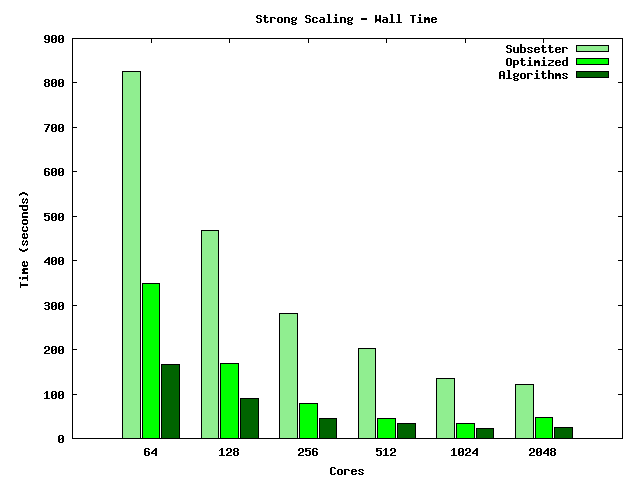
\includegraphics{strong_hist}}%
    \gplfronttext
  \end{picture}%
\endgroup

}
\caption{Strong Scaling Test.  First, the subsetter was run as a whole
program ("Subsetter").  Second, the subsetter was optimized to read less data
in the case of a subset ("Optimized").  Lastly, nearly all IO was stripped
from the program to capture the performance of the packing routines
("Algorithms").  At smaller numbers of cores, there is a greater difference
between time spent in IO and time spent everywhere else.}
\label{fig:strong}
\end{figure}

Fig. \ref{fig:strong_io} shows the IO bandwidth results of the test.  This
test captures the scalability of the IO system which correlates with the
scalability portrayed in Fig. \ref{fig:strong}.  Although in the unoptimized
case the read bandwidth may have benefited from additional cores beyond 2048,
the write bandwidth appears to have reached a plateau near 1024 processors.
The hardware is likely reaching its saturation point if not already there.
The optimized bandwidths matched those of the original subsetter given a small
amount of variability.  The notable exception is that of the optimized read
bandwidth which leveled off near 512 cores. The fact that the optimized read
tracks the unoptimized read bandwidth up to 512 processors, even though the
number of cores that are nominally reading data is smaller, reflects
optimizations in both the Parallel-NetCDF and the MPI-IO libraries that are
redistributing the reads to more processors.

\begin{figure}[!t]
\center
\resizebox{3.5in}{!}{
% GNUPLOT: LaTeX picture with Postscript
\begingroup
  \makeatletter
  \providecommand\color[2][]{%
    \GenericError{(gnuplot) \space\space\space\@spaces}{%
      Package color not loaded in conjunction with
      terminal option `colourtext'%
    }{See the gnuplot documentation for explanation.%
    }{Either use 'blacktext' in gnuplot or load the package
      color.sty in LaTeX.}%
    \renewcommand\color[2][]{}%
  }%
  \providecommand\includegraphics[2][]{%
    \GenericError{(gnuplot) \space\space\space\@spaces}{%
      Package graphicx or graphics not loaded%
    }{See the gnuplot documentation for explanation.%
    }{The gnuplot epslatex terminal needs graphicx.sty or graphics.sty.}%
    \renewcommand\includegraphics[2][]{}%
  }%
  \providecommand\rotatebox[2]{#2}%
  \@ifundefined{ifGPcolor}{%
    \newif\ifGPcolor
    \GPcolortrue
  }{}%
  \@ifundefined{ifGPblacktext}{%
    \newif\ifGPblacktext
    \GPblacktexttrue
  }{}%
  % define a \g@addto@macro without @ in the name:
  \let\gplgaddtomacro\g@addto@macro
  % define empty templates for all commands taking text:
  \gdef\gplbacktext{}%
  \gdef\gplfronttext{}%
  \makeatother
  \ifGPblacktext
    % no textcolor at all
    \def\colorrgb#1{}%
    \def\colorgray#1{}%
  \else
    % gray or color?
    \ifGPcolor
      \def\colorrgb#1{\color[rgb]{#1}}%
      \def\colorgray#1{\color[gray]{#1}}%
      \expandafter\def\csname LTw\endcsname{\color{white}}%
      \expandafter\def\csname LTb\endcsname{\color{black}}%
      \expandafter\def\csname LTa\endcsname{\color{black}}%
      \expandafter\def\csname LT0\endcsname{\color[rgb]{1,0,0}}%
      \expandafter\def\csname LT1\endcsname{\color[rgb]{0,1,0}}%
      \expandafter\def\csname LT2\endcsname{\color[rgb]{0,0,1}}%
      \expandafter\def\csname LT3\endcsname{\color[rgb]{1,0,1}}%
      \expandafter\def\csname LT4\endcsname{\color[rgb]{0,1,1}}%
      \expandafter\def\csname LT5\endcsname{\color[rgb]{1,1,0}}%
      \expandafter\def\csname LT6\endcsname{\color[rgb]{0,0,0}}%
      \expandafter\def\csname LT7\endcsname{\color[rgb]{1,0.3,0}}%
      \expandafter\def\csname LT8\endcsname{\color[rgb]{0.5,0.5,0.5}}%
    \else
      % gray
      \def\colorrgb#1{\color{black}}%
      \def\colorgray#1{\color[gray]{#1}}%
      \expandafter\def\csname LTw\endcsname{\color{white}}%
      \expandafter\def\csname LTb\endcsname{\color{black}}%
      \expandafter\def\csname LTa\endcsname{\color{black}}%
      \expandafter\def\csname LT0\endcsname{\color{black}}%
      \expandafter\def\csname LT1\endcsname{\color{black}}%
      \expandafter\def\csname LT2\endcsname{\color{black}}%
      \expandafter\def\csname LT3\endcsname{\color{black}}%
      \expandafter\def\csname LT4\endcsname{\color{black}}%
      \expandafter\def\csname LT5\endcsname{\color{black}}%
      \expandafter\def\csname LT6\endcsname{\color{black}}%
      \expandafter\def\csname LT7\endcsname{\color{black}}%
      \expandafter\def\csname LT8\endcsname{\color{black}}%
    \fi
  \fi
  \setlength{\unitlength}{0.0500bp}%
  \begin{picture}(7200.00,5040.00)%
    \gplgaddtomacro\gplbacktext{%
      \csname LTb\endcsname%
      \put(726,660){\makebox(0,0)[r]{\strut{} 0}}%
      \put(726,1336){\makebox(0,0)[r]{\strut{} 1}}%
      \put(726,2013){\makebox(0,0)[r]{\strut{} 2}}%
      \put(726,2689){\makebox(0,0)[r]{\strut{} 3}}%
      \put(726,3365){\makebox(0,0)[r]{\strut{} 4}}%
      \put(726,4042){\makebox(0,0)[r]{\strut{} 5}}%
      \put(1711,440){\makebox(0,0){\strut{}64}}%
      \put(2563,440){\makebox(0,0){\strut{}128}}%
      \put(3416,440){\makebox(0,0){\strut{}256}}%
      \put(4268,440){\makebox(0,0){\strut{}512}}%
      \put(5121,440){\makebox(0,0){\strut{}1024}}%
      \put(5973,440){\makebox(0,0){\strut{}2048}}%
      \put(220,2520){\rotatebox{90}{\makebox(0,0){\strut{}Gigabytes/second}}}%
      \put(3842,110){\makebox(0,0){\strut{}Cores}}%
      \put(3842,4710){\makebox(0,0){\strut{}Strong Scaling - IO - 48 OSTs}}%
    }%
    \gplgaddtomacro\gplfronttext{%
      \csname LTb\endcsname%
      \put(5839,4207){\makebox(0,0)[r]{\strut{}Read}}%
      \csname LTb\endcsname%
      \put(5839,3987){\makebox(0,0)[r]{\strut{}Write}}%
    }%
    \gplbacktext
    \put(0,0){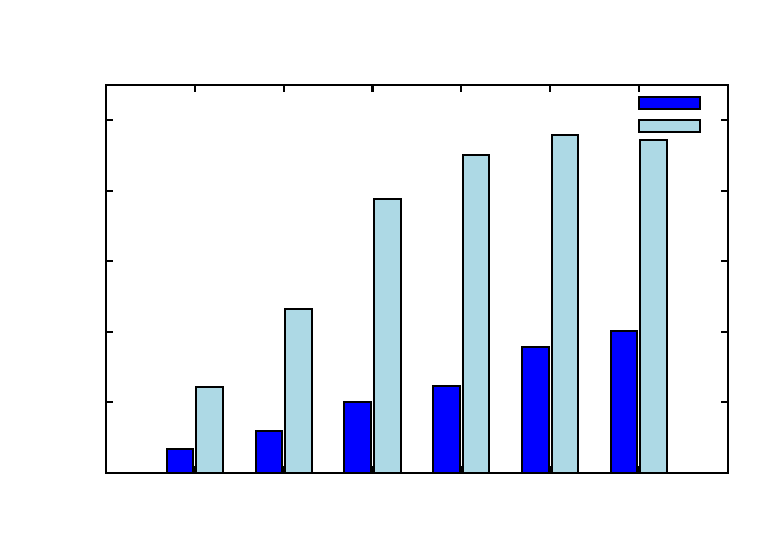
\includegraphics{strong_io_hist}}%
    \gplfronttext
  \end{picture}%
\endgroup

}
\caption{Strong Scaling Test for IO Bandwidth.  The Read and Write bandwidths
are compared as the number of cores are increased.  The subsetter and its
optimized versions are both shown.  In general, all bandwidths increased with
respect to the number of cores.  The optimized bandwidths matched those of the
original subsetter given a small amount of variability.  The notable exception
is that of the optimized read bandwidth which leveled off near 512 cores.}
\label{fig:strong_io}
\end{figure}

Table \ref{tab:strong_prof} represents a profile for process zero for the 2048
process run.  The function names are sufficiently self-documenting for those
familiar with C++ syntax.  The zeroth process represents a worst-case scenario
since the default distribution of data using GA will always put data on at
least the zeroth process implying process zero should have at least as much
work to perform as any other processor.  The profile for the 2048 run was
selected arbitrarily, however the profiles for the other strong scaling runs
(not shown) demonstrated a similar trend.  The functions which did not
contribute a significant amount of time to the program were removed and the
table is sorted by total time spent in the function.  The number of calls to
the read and write routines were small.  (Not shown in Table
\ref{tab:strong_prof} is the number of calls to the function comparing each
latitude/longitude pair to the desired subset region which accounts for over
60\% of the function calls.)  However, the amount of time spent in the read
and write routines was significant.  In all cases, the amount of time spent in
IO was at least 75\% of the program's execution.  IO is clearly the dominant
factor in running our code.

\begin{table*}[!t]
\center
\caption{Partial Profile for Process 0 at 2048 Cores - MJO Region}
\label{tab:strong_prof}
\begin{tabular}{lrrrrrr}
Name&Calls&Percent Calls&Time (seconds)&Percent Time&Time/call (seconds)\\
NetcdfVariable::read()                    &39&0.1&156.1&93.0&4.00\\
NetcdfFileWriter::write(int,int,int)      &34&0.1&  5.9& 3.5&0.17\\
VariableDecorator::read()                 & 5&0.0&  1.7& 1.0&0.34\\
NetcdfDataset::NetcdfDataset(string)      & 5&0.0&  1.2& 0.7&0.24\\
Dataset::adjust\_masks(LatLonBox)         & 1&0.0&  1.0& 0.6&1.05\\
ConnectivityVariable::reindex()           & 3&0.0&  0.7& 0.4&0.25\\
NetcdfFileWriter::NetcdfFileWriter(string)& 1&0.0&  0.2& 0.2&0.29\\
\end{tabular}
\end{table*}

Table \ref{tab:strong_prof_opt} represents a profile for process zero for the
2048 process run using the optimized subsetter.  The notable differences
between Table \ref{tab:strong_prof_opt} and Table \ref{tab:strong_prof} are
the total time and percentage of time spent in each function.  Although the
optimized subsetter spends substantially less time reading, the majority of
time is still spent in IO.  Although still dominant, IO is a less significant
contributor to the total execution time.

\begin{table*}[!t]
\center
\caption{Partial Profile for Process 0 at 2048 Cores - MJO Region - Optimized}
\label{tab:strong_prof_opt}
\begin{tabular}{lrrrrrr}
Name&Calls&Percent Calls&Time (seconds)&Percent Time&Time/call (seconds)\\
NetcdfVariable::read()                    & 39&0.1&22.8&65.4&0.58\\
NetcdfFileWriter::write(int,int,int)      & 34&0.1& 6.5&18.7&0.19\\
NetcdfDataset::NetcdfDataset(string)      &  5&0.0& 1.2& 3.4&0.24\\
VariableDecorator::read()                 &  5&0.0& 1.1& 3.0&0.21\\
Dataset::adjust\_masks(LatLonBox)         &  1&0.0& 0.8& 2.4&0.82\\
ConnectivityVariable::reindex()           &  3&0.0& 0.8& 2.2&0.26\\
NetcdfFileWriter::NetcdfFileWriter(string)&  1&0.0& 0.4& 1.1&0.37\\
\end{tabular}
\end{table*}

\subsection{Discussion}

Running our subsetter at a scale of over 2000 cores is initially promising.
Fig. \ref{fig:strong} demonstrates that the algorithms we developed scale
to at least 1024 processors.  The performance of the original subsetter
can be considered as the case where operations on the entire globe are
performed. For these operations, the subsetter would be reading
all of the available data.  These global subset will stress the IO system
the greatest.  The optimized subsetter will not help in cases of operations on
the entire globe.  The significant improvement
afforded by the optimized subsetter is likely due to both the data layout using a
space-filling curve as explained in Section \ref{subsection:grid} and
optimization of collective read operations in both the Parallel-NetCDF and
MPI-IO libraries.  The
space-filling curve places logically adjacent cells near each other in memory
allowing for the maximum number of nonparticipating processes during the read
operation.

The profile of the global reads in Table \ref{tab:strong_prof} suggests that
IO accounts for nearly 95\% of program execution at 2048 cores.  This is not a
stretch of the imagination since our software reads, subsets, and then writes.
Even if our code performed a significant calculation after each read of the
edge variable, the profile would likely remain IO bound.  At fewer numbers of
cores the percentage of time spent in IO ranged from 75\% to the 95\% shown in
Table \ref{tab:strong_prof}.  Even in the optimized case, the profile remains
IO bound.

The reason for the disproportionately faster write bandwidth versus read
bandwith seen in Fig. \ref{fig:strong_io} is probably due to caching by the
Lustre parallel filesystem.  The relatively small amount of data being written
is most likely being copied to an internal buffer allowing the functions to
return quickly.

\section{Future Work}
\label{section:future}

The success of the NetCDF Operators\cite{NCO} and similar tools demonstrate
the need for user-ready applications for the analysis of their users' data.
The success of tools such as CDAT\cite{CDAT} validate the need for a
scriptable interface and customization of basic and advanced operators.  We
plan to provide both the scriptable interface as well as a set of predefined
command-line tools.

We are currently developing a general C++ API for climate data analysis in a
data parallel fashion based on the PGAS model and one-sided communications.
The API will be leveraged to produce additional command-line tools, however it
is intended primarily to be used by climate scientists to produce the kinds of
tailored analyses which they require.  Time permitting, the API will be
exposed to the Python language in order to facilitate ease of use in a
scripted environment.  Larson, Ong, and Tokarz also point out certain
capabilities missing from popular climate data analysis packages such as
probability density function (PDF) estimation as well as the sorting and
ordering of data.

The evaluation performed in Section \ref{section:evaluation} revealed that IO
for our application remains the greatest bottleneck.  This fact is exacerbated
when large regions representing the entire grid are subset.  Our current
optimized strategy of reading chunks of variables based on whether a process
participates in the later subset still reads more data than is eventually
redistributed.  If a masked read or a read based on individual array index
tuples similar to \verb+NGA_Gather+ were available within the Parallel-NetCDF
library we might see further performance gains.  The algorithms presented in
this paper which evenly distribute the subset data will hopefully encourage
work in this area.  We are also investigating recent advances in the
Parallel-NetCDF library \cite{PNETCDFOPT} which addresses the limitation in
the current interface of only allowing access to one array variable per
function call.

\section{Conclusion}
\label{section:conclusion}

We developed a novel data parallel subsetter of climate data based on
unstructured grids, the PGAS programming model, and one-sided communication.
The experimental evaluation showed scalability to thousands of processors and
acceptable IO bandwidth.  IO bandwidth is the greatest bottleneck in scaling
these types of applications.

\section*{Acknowledgment}
The authors are indebted to Wei-keng Liao at Northwestern University for
invaluable help in getting the subsetter running and optimized on the Franklin
platform.

This research was funded by the U.S. Department of Energy's (DOE) Office of
Advanced Scientific Computing Research through its Scientific Discovery
through Advanced Computing program and was performed at DOE's National Energy
Research Scientific Computing Center.


% trigger a \newpage just before the given reference
% number - used to balance the columns on the last page
% adjust value as needed - may need to be readjusted if
% the document is modified later
%\IEEEtriggeratref{16}
% The "triggered" command can be changed if desired:
%\IEEEtriggercmd{\enlargethispage{-5in}}

% references section

\bibliographystyle{IEEEtran}
\bibliography{IEEEabrv,paper}

% that's all folks
\end{document}
